\section{Improved Electron-Jet Overlap Removal}

\begin{frame}
    \frametitle{Improved Electron-Jet Overlap Removal}
\begin{columns}
\column{.5\textwidth}
\begin{figure}
\centering
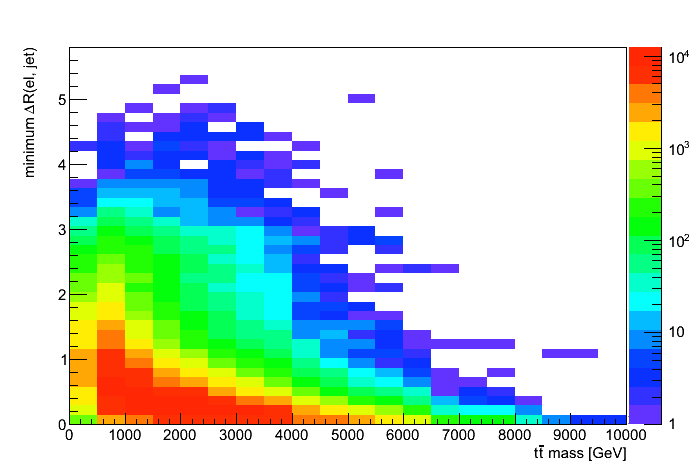
\includegraphics[width=\textwidth]{dR_e_jet_mtt.png}
\end{figure}
\column{.5\textwidth}
\begin{itemize}
    \item The angular separation between the lepton and $b$ quark falls at
        high \mtt\ since $\dr(b,W) \sim 1/p_T^{top}$.
    \item Jets are built from energy deposits in both the EM and
        hadronic calorimeters.
    \item If electron and $b$ quark separated by $\dr < R_{jet}$,
        resulting jet often includes energy from both particles
    \item Double counting of energy in \mtt\ reconstruction!
\end{itemize}
\end{columns}
\end{frame}

\subsection{Procedures}

\begin{frame}
    \frametitle{Procedure}
\begin{itemize}
    \item OLD procedure: remove one object if \smallr\ jet and
        electron separated by $\dr < 0.4\ \to$ loss in efficiency
    \item NEW procedure:
    \begin{itemize}
        \item select electrons
        \item if any electron and jet separated by $\dr < 0.4$,
            subtract electron four-momentum from nearest jet
        \item select jets in the event after this subtraction
        \item if electron still within $\dr < 0.2$ of a selected jet,
            remove electron and restore original jet four-momentum
    \end{itemize}
\end{itemize}
\end{frame}

\begin{frame}
    \frametitle{Procedure}
\begin{figure}
\centering
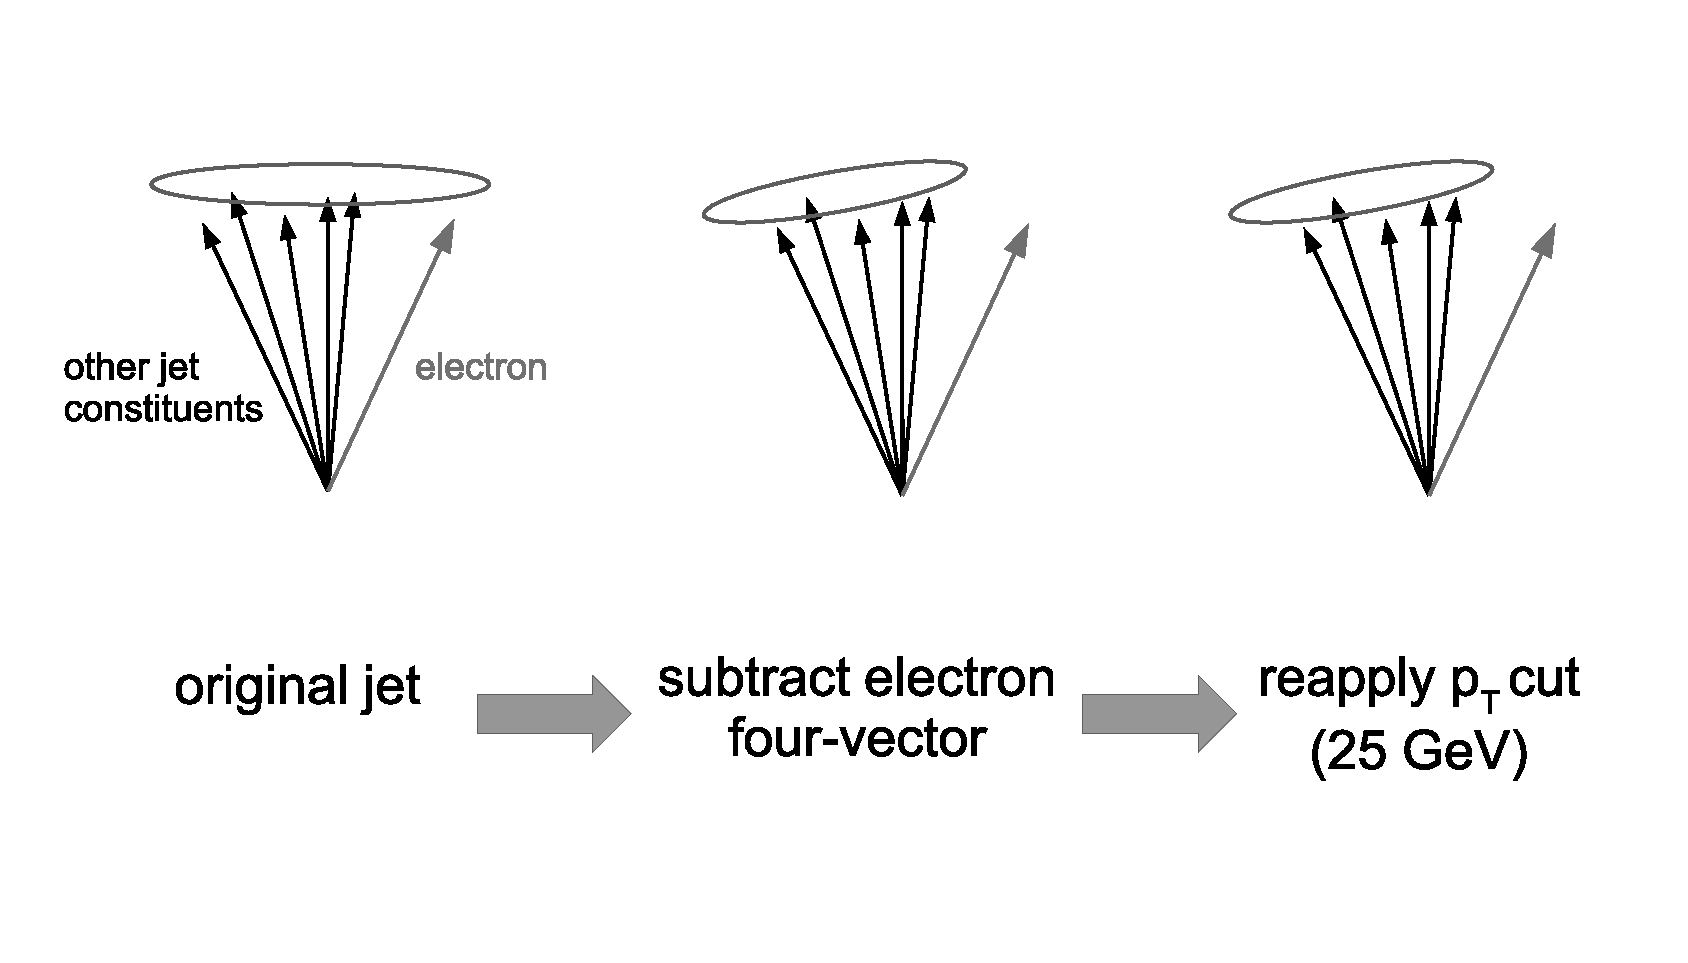
\includegraphics[width=\textwidth]{schematic.eps}
\end{figure}
\end{frame}

\subsection{Jet Performance}

\begin{frame}
    \frametitle{Jet Performance}
It is important that jets undergoing the overlap procedure (left) have
similar $p_T$ resolution after the procedure to those unaffected by it
(right).
\begin{figure}
\centering
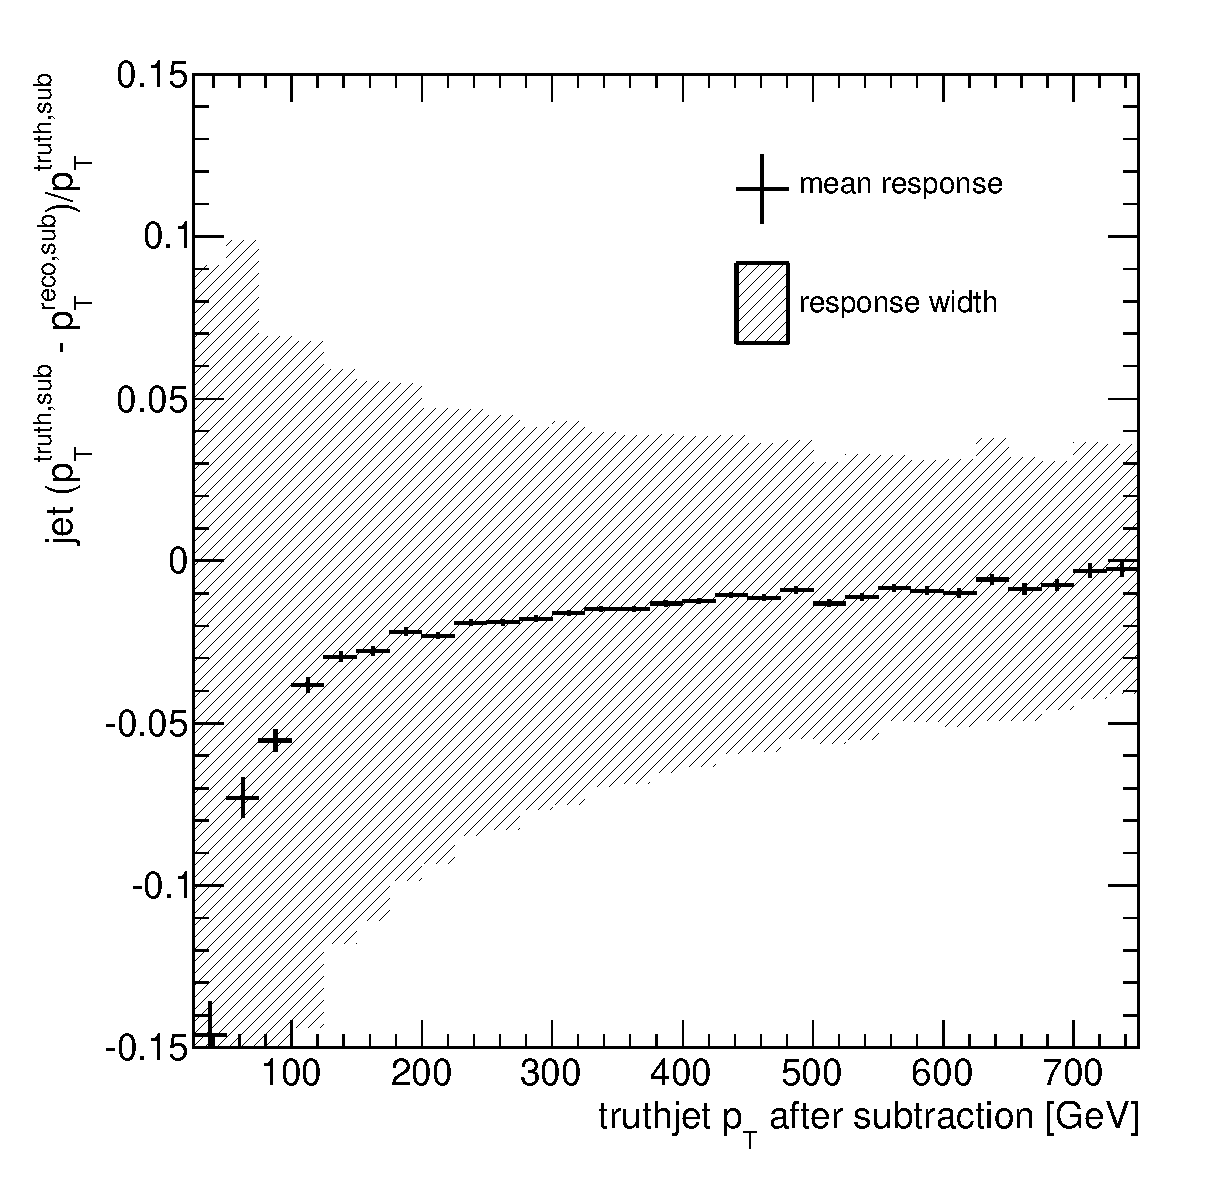
\includegraphics[width=.5\textwidth]{jet_reso_sub.eps}
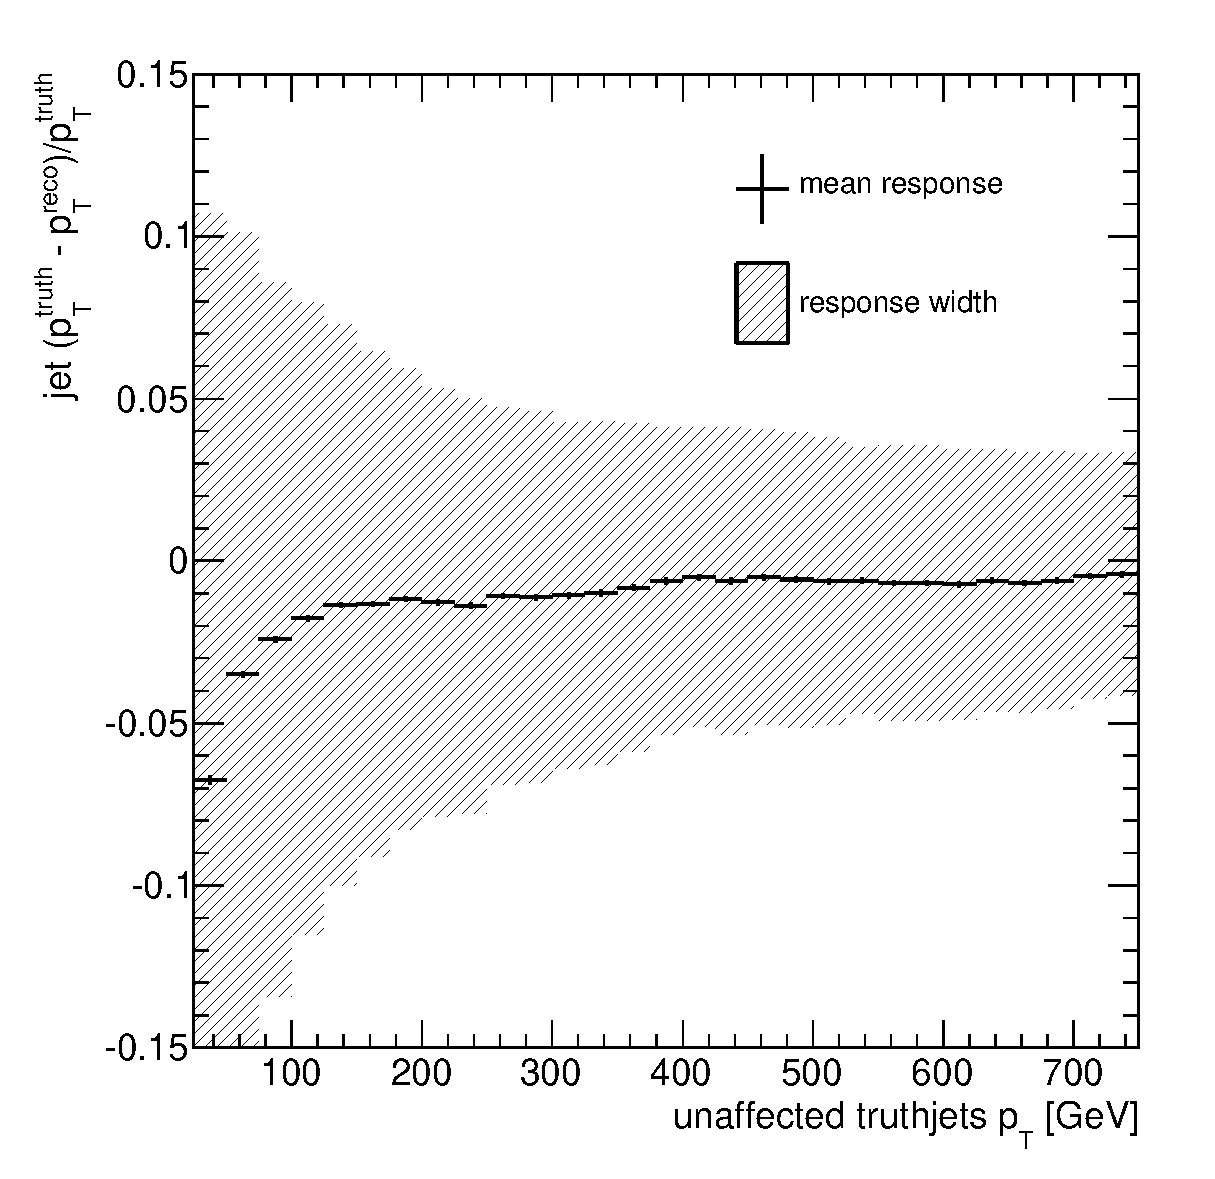
\includegraphics[width=.5\textwidth]{jet_reso_unaffected.eps}
\end{figure}
\end{frame}

\subsection{Electron Efficiency Corrections}

\begin{frame}
    \frametitle{Electron Efficiency Corrections}
It is also important that the efficiency of electrons undergoing the
overlap procedure is well-modeled by simulation.
\begin{figure}
\centering
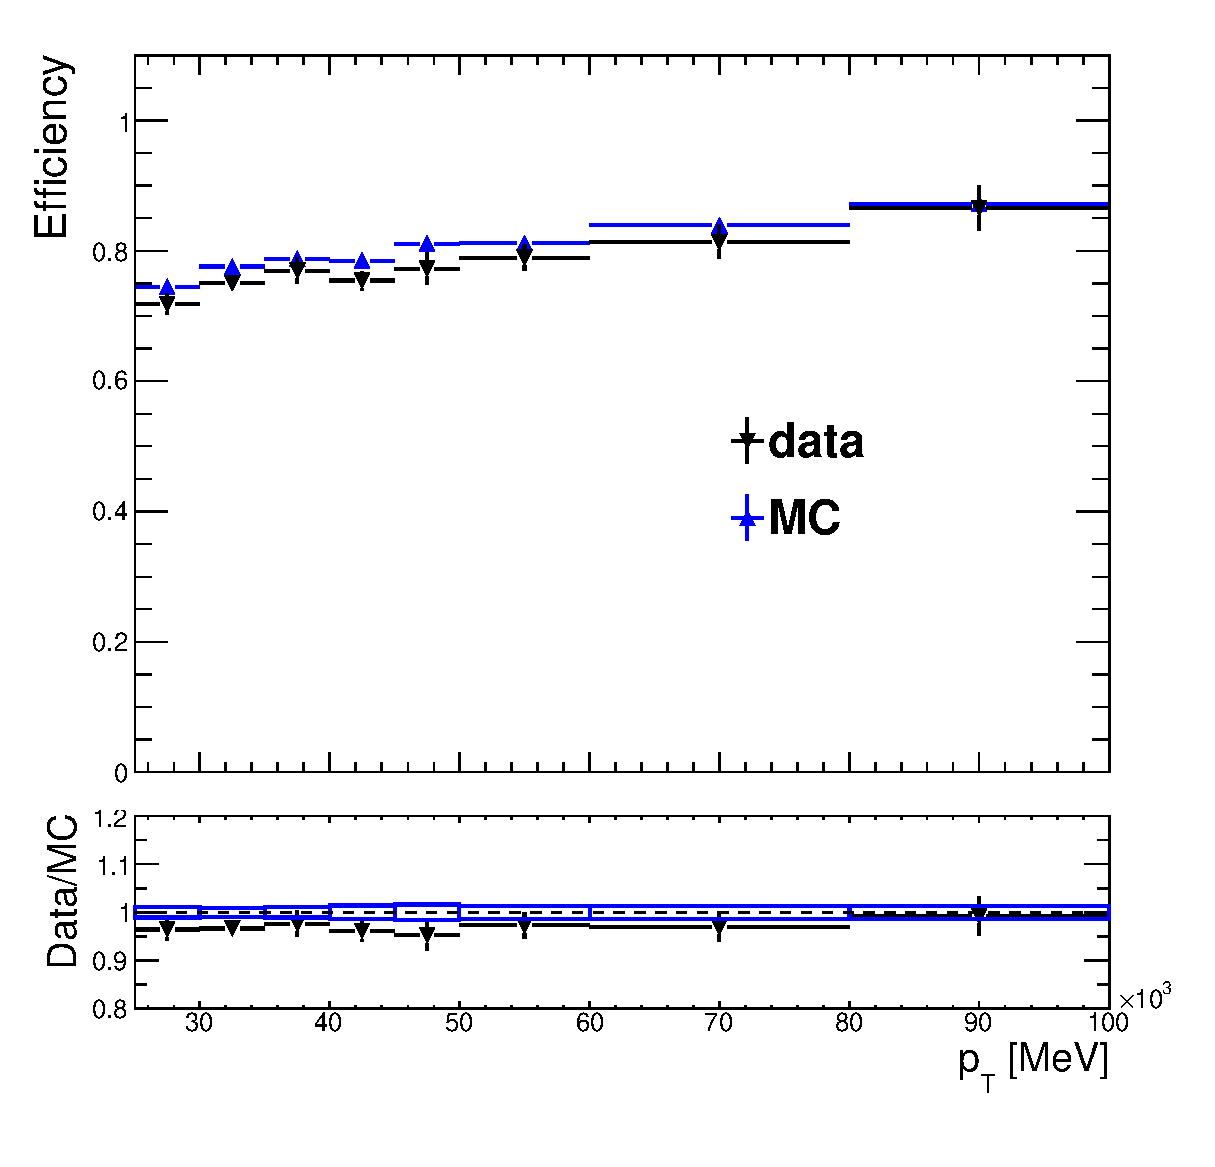
\includegraphics[width=.5\textwidth]{tightpp_nearjets_pt_sf.eps}
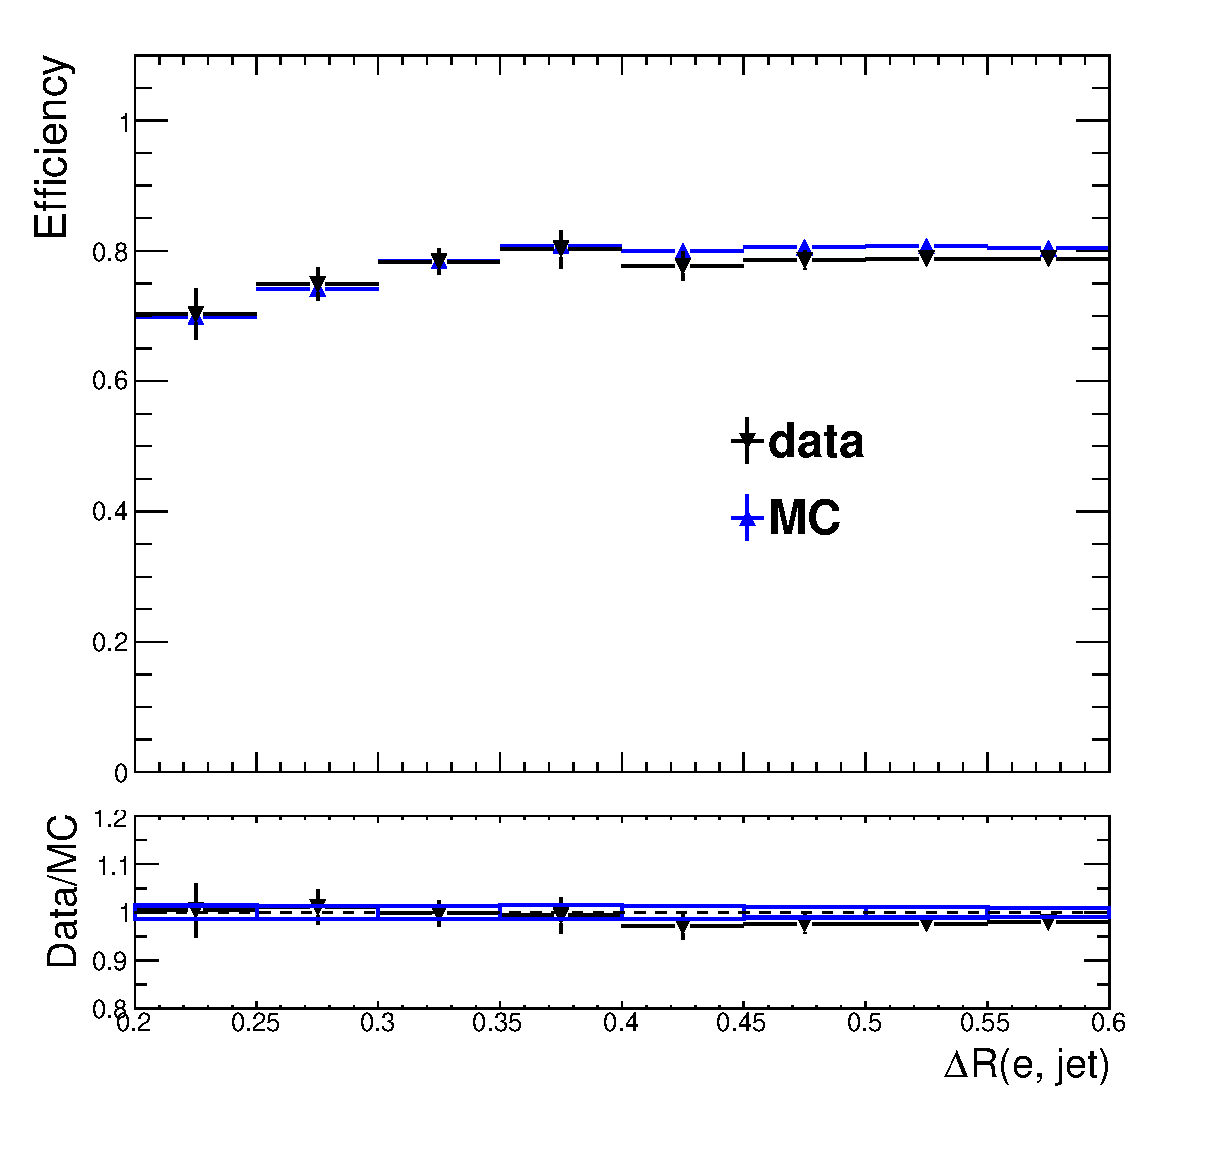
\includegraphics[width=.5\textwidth]{tightpp_nearjets_drjet_sf.eps}
\end{figure}
\end{frame}

\subsection{Efficiency Improvements}

\begin{frame}
    \frametitle{Efficiency Improvements}
\begin{columns}
\column{.5\textwidth}
\centering
OLD selection efficiency
\begin{figure}
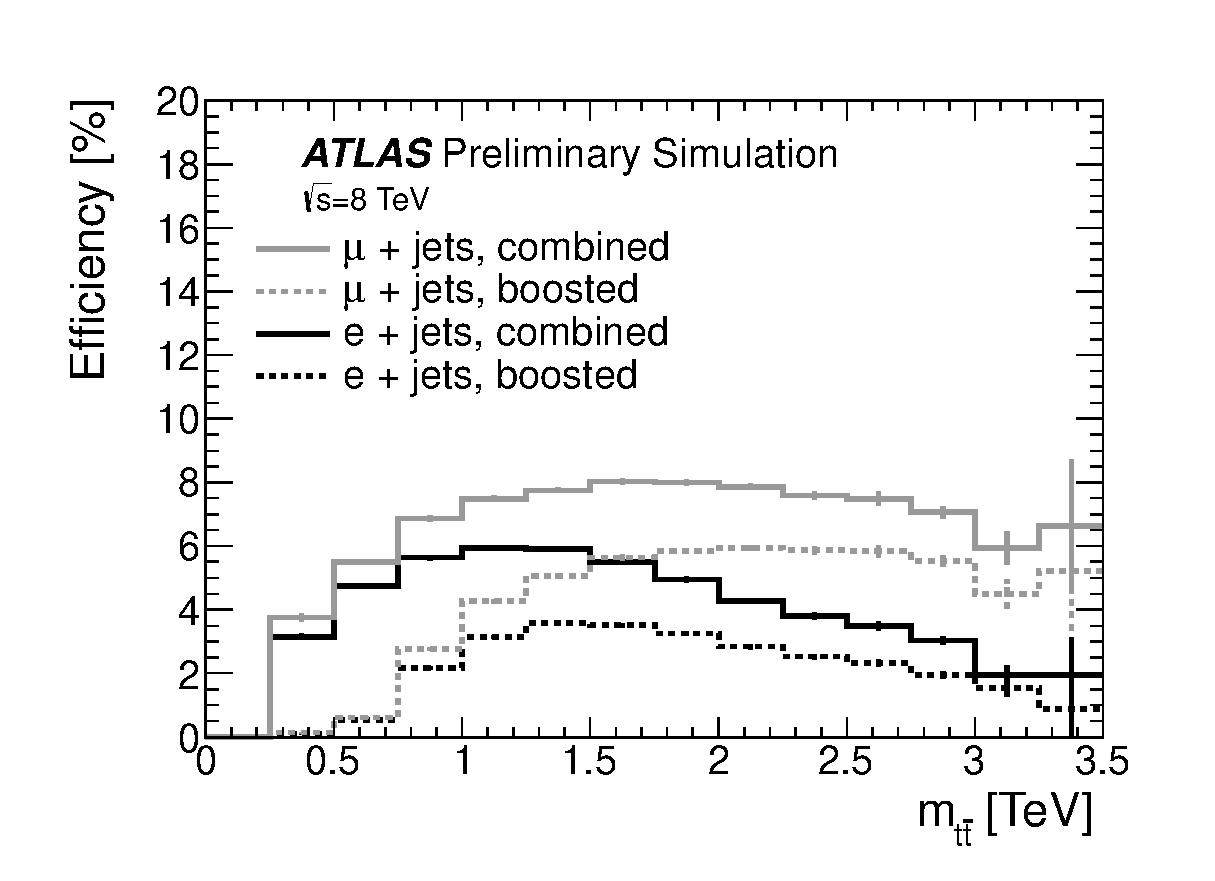
\includegraphics[width=\textwidth]{selectionefficiency.eps}
\end{figure}
\column{.5\textwidth}
\centering
NEW selection efficiency
\begin{figure}
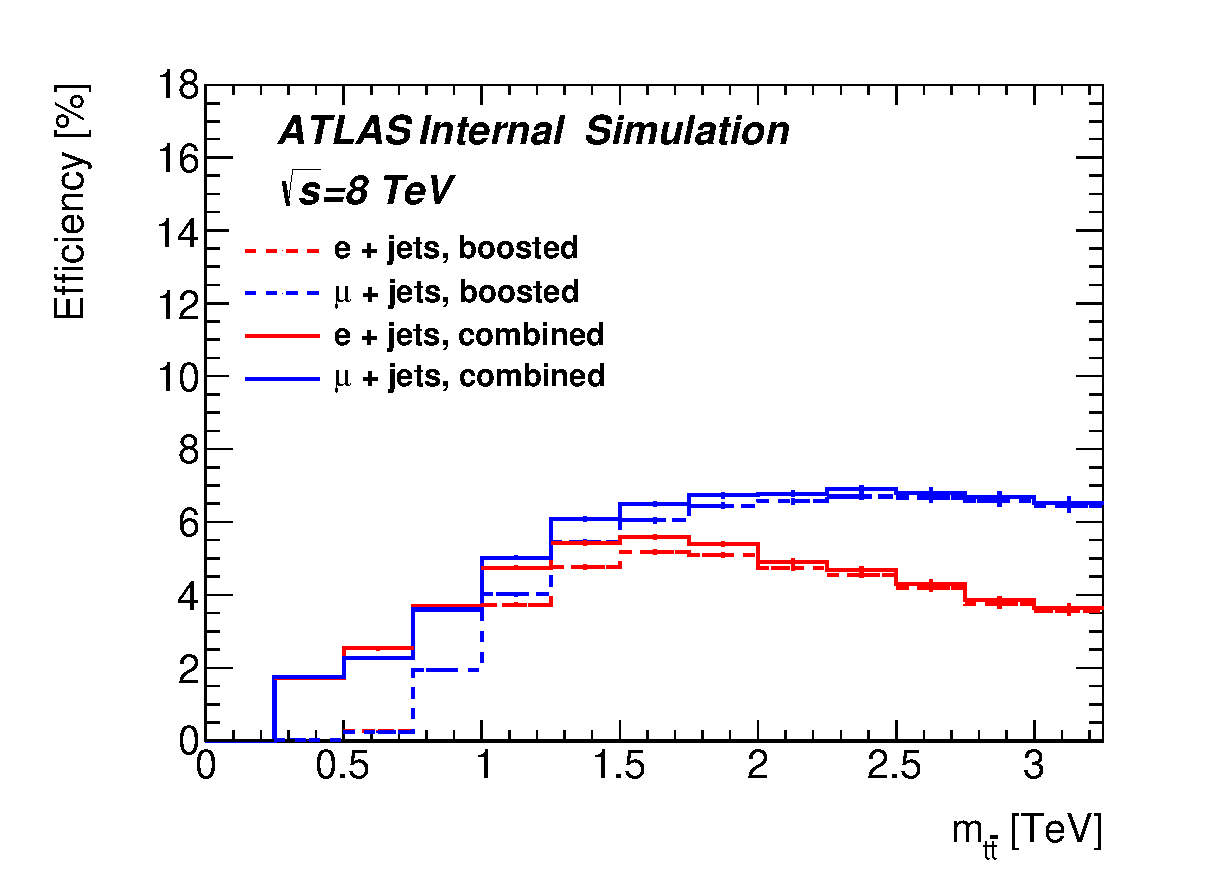
\includegraphics[width=\textwidth]{neweff.eps}
\end{figure}
\end{columns}

\centering
\vspace{15pt}
This translates to 33\% and 51\% efficiency improvements for \\
2.5 and 3.0~TeV $\zp_{topcolor}$ resonances.
\end{frame}
